%Argonne 2023 May 18 Argonne Talk
\documentclass[10pt,compress,xcolor={usenames,dvipsnames},aspectratio=169]{beamer}
%\usepackage[T1]{fontenc}
%\usepackage{tgadventor} %Font found at https://tug.org/FontCatalogue/
%\usepackage{newpxtext}
\usepackage{newtxtext}
%\usepackage[light]{antpolt}
\usepackage[T1]{fontenc}
\usepackage{datetime2}
%\usepackage[euler-digits,euler-hat-accent]{eulervm}


\usepackage{amsmath,
	amssymb,
	datetime,
	mathtools,
	bbm,
	%mathabx,
	array,
	booktabs,
	xspace,
	multirow,
	calc,
	colortbl,
	siunitx,
	centernot,
 	graphicx}
\usepackage[usenames]{xcolor}
\usepackage[giveninits=false,
backend=biber,
style=nature,
style=authoryear-comp,
maxcitenames=4,
mincitenames=2]{biblatex}
\addbibresource{FJHown23.bib}
\addbibresource{FJH23.bib}
\usepackage{media9}
\usepackage[autolinebreaks]{mcode}
\usepackage[tikz]{mdframed}
\graphicspath{{figures/}}


\usetheme{FJHSlimNoFoot169}
\setlength{\parskip}{2ex}
\setlength{\arraycolsep}{0.5ex}
\setbeamertemplate{itemize subitem}[triangle]
\setbeamerfont{footnote}{size=\scriptsize}

\DeclareMathOperator{\SOL}{SOL}
\DeclareMathOperator{\APP}{APP}
\DeclareMathOperator{\ERR}{ERR}
\DeclareMathOperator{\AVG}{AVG}
\DeclareMathOperator{\INT}{INT}
\DeclareMathOperator{\LIN}{LINEAR}
\DeclareMathOperator{\BAD}{BAD}
\DeclareMathOperator{\DISC}{DSC}
\DeclareMathOperator{\VAR}{VAR}
\DeclareMathOperator{\CONF}{CNF}
%\DeclareMathOperator{\opt}{opt}
\newcommand{\dataN}{\bigl(\hf(\vk_i)\bigr)_{i=1}^n}
\newcommand{\dataNj}{\bigl(\hf(\vk_i)\bigr)_{i=1}^{n_j}}
\newcommand{\dataNjd}{\bigl(\hf(\vk_i)\bigr)_{i=1}^{n_{j^\dagger}}}
\newcommand{\ERRN}{\ERR\bigl(\dataN,n\bigr)}
\newcommand{\otod}{\ensuremath{1\mkern-4mu : \mkern-2mu d}}


\iffalse
Title:  Faster Monte Carlo via Low Discrepancy Sampling
Speaker:  Fred J. Hickernell, Illinois Institute of Technology

Abstract:  Estimating an expectation or integral is important in high energy physics, Bayesian inference, image rendering, quantitative finance, and uncertainty quantification.  Monte Carlo type methods are commonly used.  The numerical error can be expressed as a product of three quantities: one measuring the deficit in the sampling scheme, a second measuring the roughness of the function defining the expectation or integral, and a third representing the confounding between that function and the sampling deficit.  We explain how low discrepancy sampling, also known as the quasi-Monte Carlo method, can substantially improve the efficiency of these calculations.  We discuss how to improve efficiency via transformations of the integral.  Our data-driven error bounds advise the user when to stop simulating.  We illustrate low discrepancy sampling via our QMCPy software library (qmcpy.org).

Bio: Fred J. Hickernell is Professor of Applied Mathematics and Vice Provost for Research at Illinois Institute of Technology.  Although his father and brothers are physicists, Fred's physical intuition was lacking so he pursued a PhD in applied mathematics.  For the past three decades, Fred has explored how to improve the efficiency of Monte Carlo methods through low discrepancy sampling, also known as the quasi-Monte Carlo method.  Recently, he and his collaborators have developed data-driven error bounds for quasi-Monte Carlo methods and have been encouraging greater application of quasi-Monte Carlo methods through the QMCPy software library.

\fi

%\DeclareMathOperator{\app}{app}

\providecommand{\HickernellFJ}{H.\xspace}
\DeclareMathOperator{\RMS}{RMS}


\renewcommand{\OffTitleLength}{-12ex}
\setlength{\FJHThankYouMessageOffset}{-8ex}
\title{Speedy Simulations}
\author[]{Sou-Cheng Choi and Fred J. Hickernell}
\institute{Illinois Institute of Technology \\
    Dept Applied Math \quad
	Ctr Interdisc Scientific Comput \quad Office of Research\\
 \href{mailto:schoi32@iit.edu}{\url{schoi32@iit.edu}}
	\\
	\href{mailto:hickernell@iit.edu}{\url{hickernell@iit.edu}} \qquad
	\href{https://sites.google.com/iit.edu/fred-j-hickernell}{\url{sites.google.com/iit.edu/fred-j-hickernell}}}

\thanksnote{Looking forward to working with you this summer \\
Slides at  \href{https://speakerdeck.com/fjhickernell/argonne2023maytalk}%
{\nolinkurl{speakerdeck.com/fjhickernell/argonne2023maytalk}} \\
Jupyter notebook with computations and figures \href{https://github.com/QMCSoftware/QMCSoftware/blob/develop/demos/talk_paper_demos/Argonne_Talk_2022_May/Argonne_2023_Talk_Figures.ipynb}{\beamerbutton{here}}\quad Visit us at \href{https://qmcpy.org}{\nolinkurl{qmcpy.org}}}

\event{SURE Kickoff}
\date[]{ revised \today}

\input FJHDef.tex

	\newcommand{\scoop}[1]{\parbox{#1}{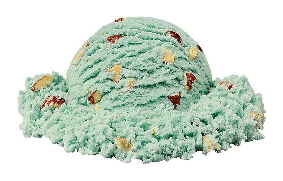
\includegraphics[width=#1]{IceCreamScoop.eps}}\xspace}
\newcommand{\smallscoop}{\scoop{1cm}}
\newcommand{\medscoop}{\scoop{1.8cm}}
\newcommand{\largescoop}{\scoop{3cm}}
\newcommand{\ICcone}[1]{\parbox{#1}{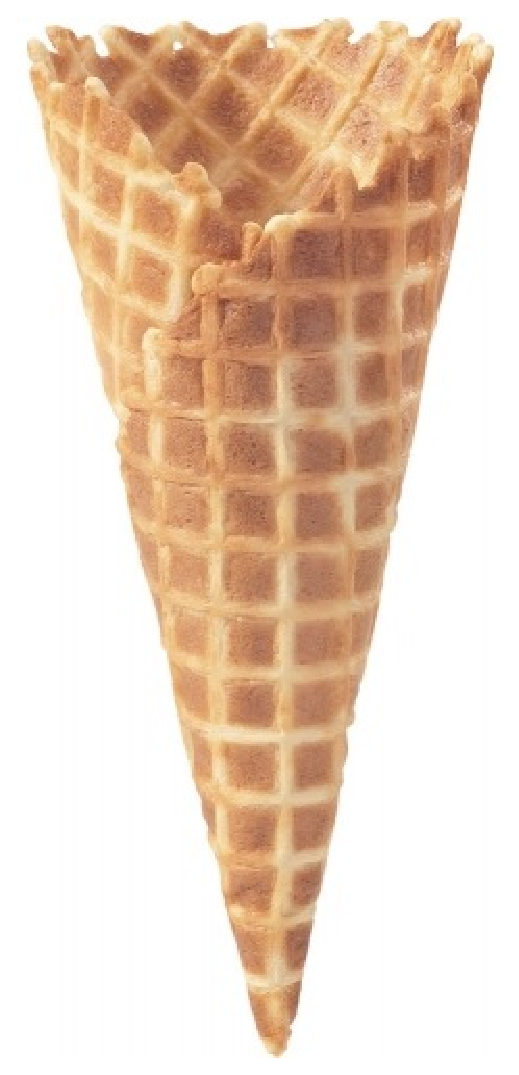
\includegraphics[width=#1,angle=270]{MediumWaffleCone.eps}}\xspace}
\newcommand{\medcone}{\ICcone{1.2cm}}
%\newcommand{\medcone}{\parbox{1.1cm}{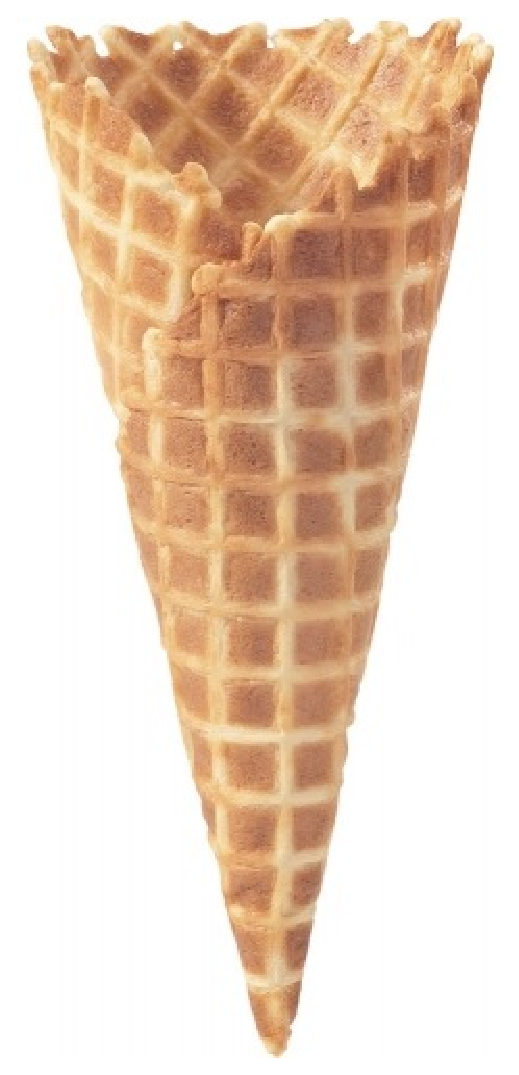
\includegraphics[width=1.2cm,angle=270]{MediumWaffleCone.eps}}\xspace}
\newcommand{\largercone}{\parbox{2.2cm}{\vspace*{-0.2cm}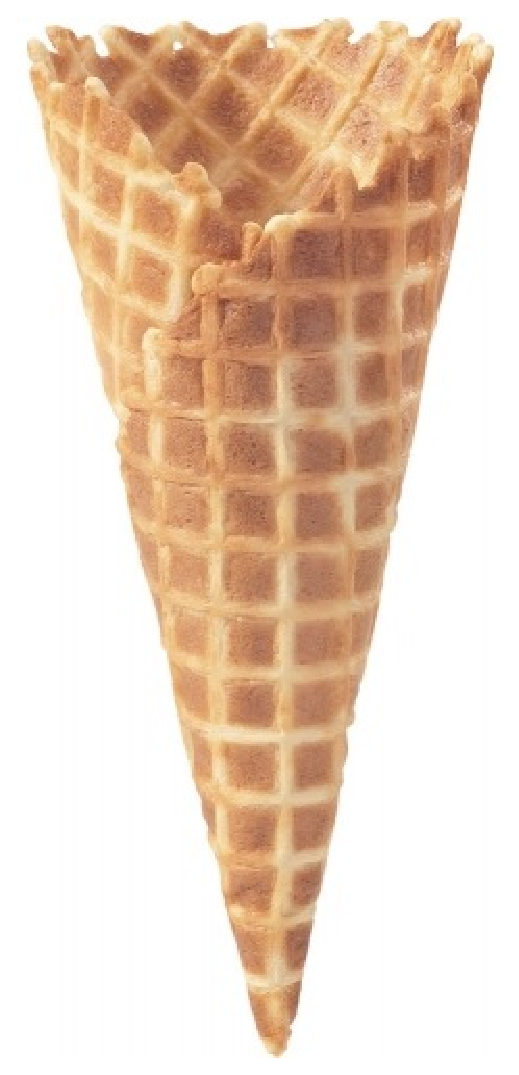
\includegraphics[width=1cm,angle=270]{MediumWaffleCone.eps}}\xspace}
\newcommand{\hugecone}{\parbox{4cm}{\vspace*{-0.2cm}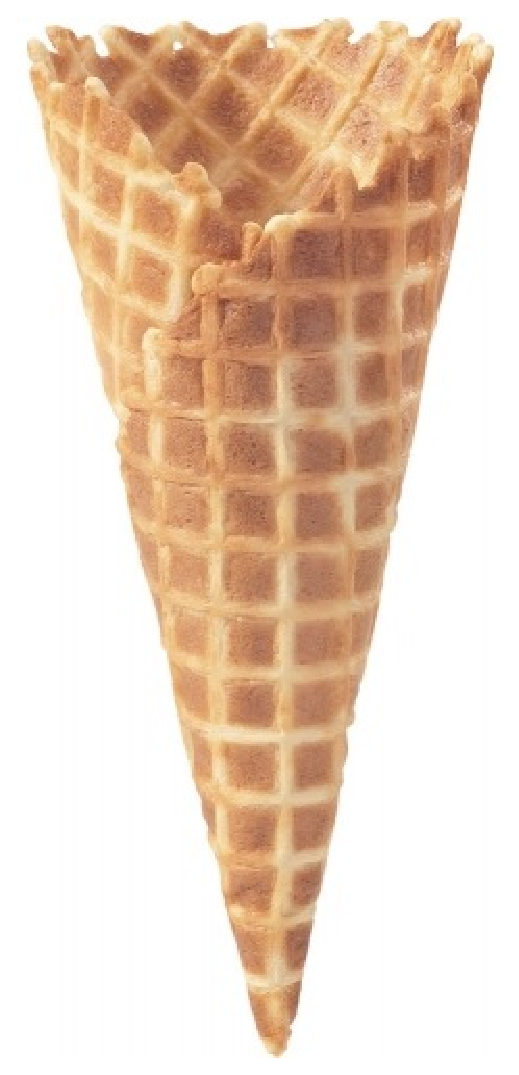
\includegraphics[width=1.8cm,angle=270]{MediumWaffleCone.eps}}\xspace}
\newcommand{\largecone}{\ICcone{1.8cm}}
\newcommand{\smallcone}{\parbox{1.1cm}{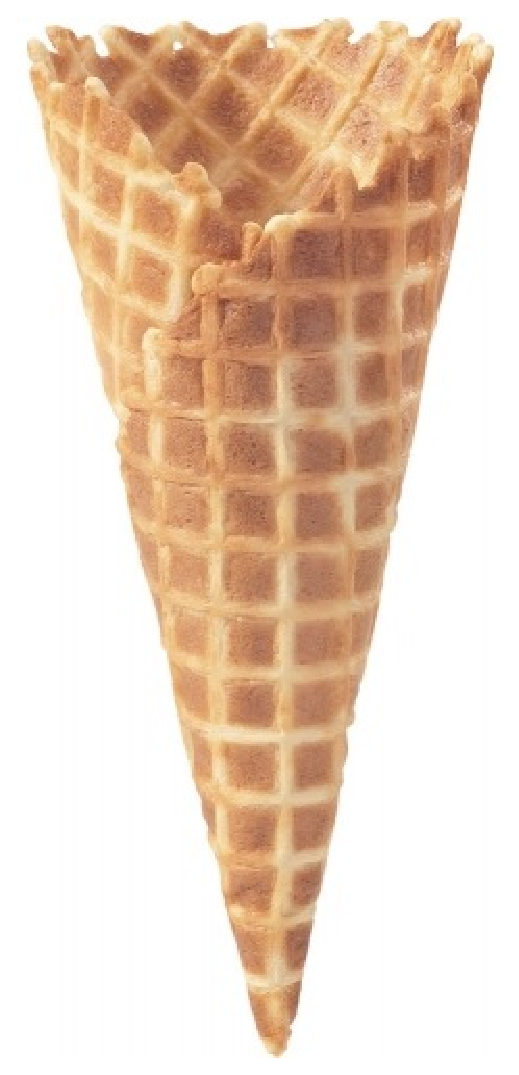
\includegraphics[width=0.5cm,angle=270]{MediumWaffleCone.eps}}\xspace}


\begin{document}
	\everymath{\displaystyle}

\frame{\titlepage}

%%%%%%%%%%%%%%%%%%%%%%%%%%%%%%%%%%%%%%%%%%
%%%%%%%%%%%%%%%%%%%%%%%%%%%%%%%%%%%%%%%%%%
\section{Why Quasi-Monte Carlo Is Faster than Simple Monte Carlo}
%%%%%%%%%%%%%%%%%%%%%%%%%%%%%%%%%%%%%%%%%%
%%%%%%%%%%%%%%%%%%%%%%%%%%%%%%%%%%%%%%%%%%


\begin{frame}{Uncertainty in a Cantilevered Beam\footfullcite{ParSee22a}}
	\vspace{-4ex}
	\begin{tabular}{m{0.6\textwidth}m{0.4\textwidth}}
		\[
		\begin{aligned}
			u(x) & = g(\vZ, x) = \text{beam deflection} \\
			x &= \text{position} \\
			& = \text{solution of a differential equation boundary value problem} \\
			\vZ & \sim \cu[1,1.2]^3 \quad \text{defines uncertainty in Young's modulus}
                & = \text{the randomness in the problem}\\
			\mu(x) &= \text{expected or mean value of the beam deflection} \\
                    & = \Ex[g(\vZ,x)] = \int_{[0,1]^3}  g(\vz,x) \, \dif \vz \approx 
                    \underbrace{\frac 1n \sum_{i=1}^n g(\vZ_i,x)}_{\substack{\text{\alert{sample mean} or }\\ \text{\alert{Monte Carlo estimate}}}}
			\\
			& \mu(\text{end}) = 1037  \qquad \text{\alert{How?}}
		\end{aligned}
		\]
		&
		\centering
		\vspace{1.5ex}
		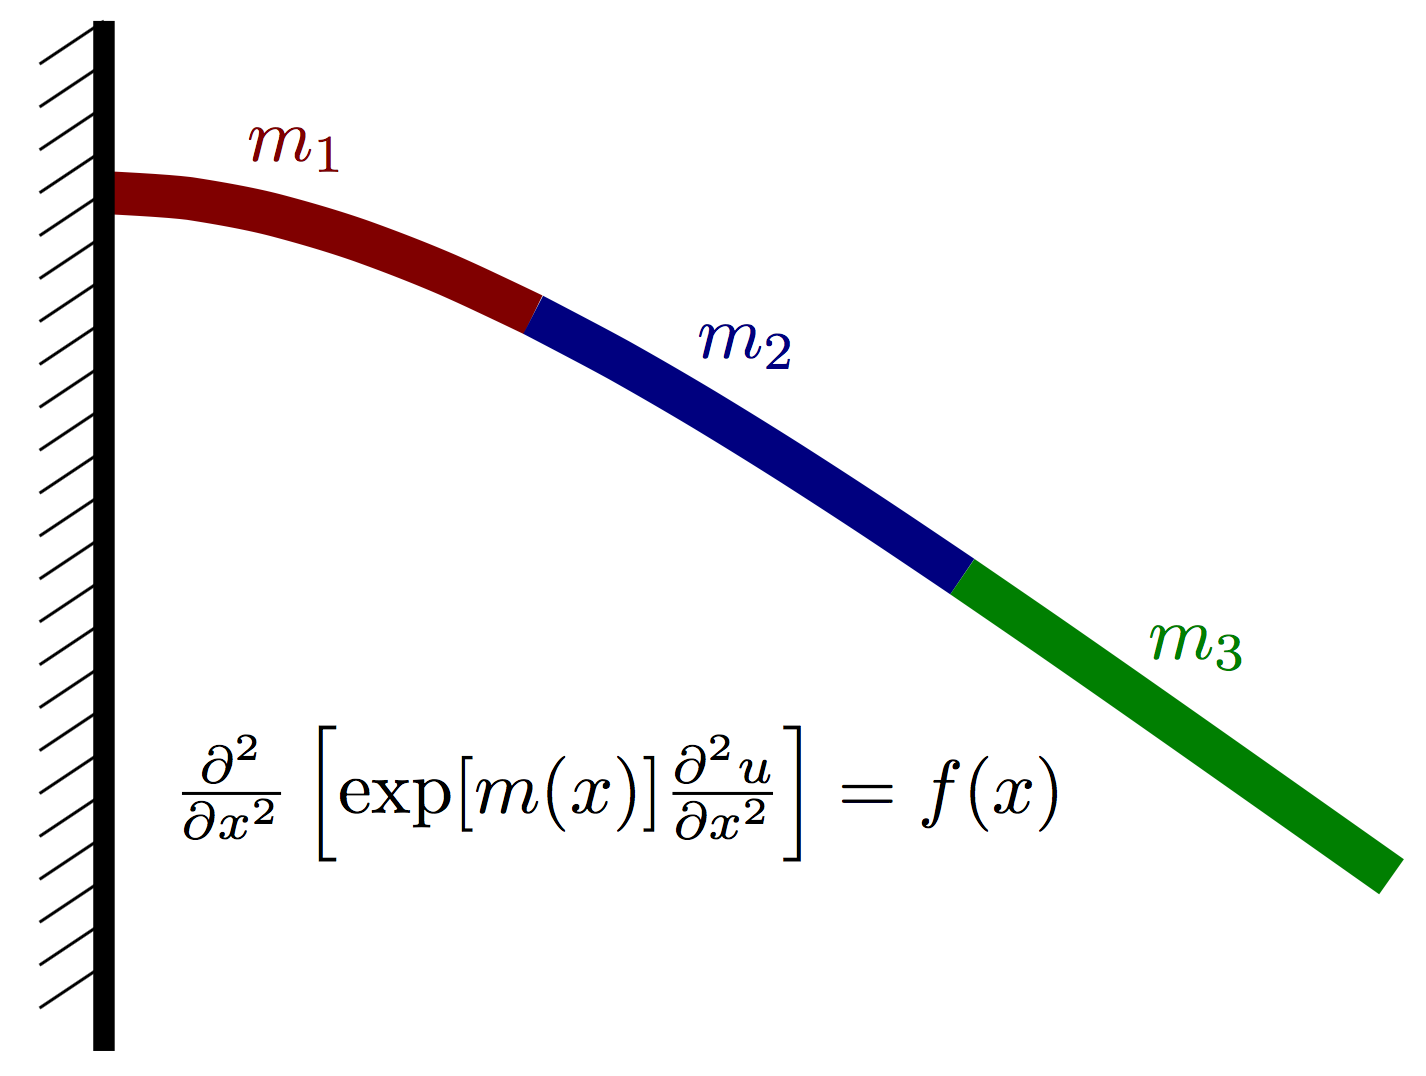
\includegraphics[width=0.35\textwidth]{BeamDrawing.png} \newline
	\end{tabular}


\end{frame}


\begin{frame}{IID vs.\ Low Discrepancy for the Cantilevered Beam via QMCPy\footfullcite{QMCPy2020a}}
	\vspace{-3ex}
	\begin{tabular}{m{0.63\textwidth}m{0.35\textwidth}}
		\[
		\begin{aligned}
				g(\vZ, x) &= \text{beam deflection} \\
			\only<1>{\vZ & \sim \cu[1,1.2]^3 \quad \text{defines uncertainty} \\
			x &= \text{position} \\}
			\mu(x) &= \Ex[g(\vZ, x)] &
			\mu(\text{end}) &= 1037
		\end{aligned}
		\]
  	\vspace{-11ex}\only<2>{\vspace{-3ex}}
	\includegraphics<1>[width=0.6\textwidth]{iidldbeam.eps}
	\includegraphics<2>[width=0.65\textwidth]{ldparallelbeam.eps}
		&
		\centering
		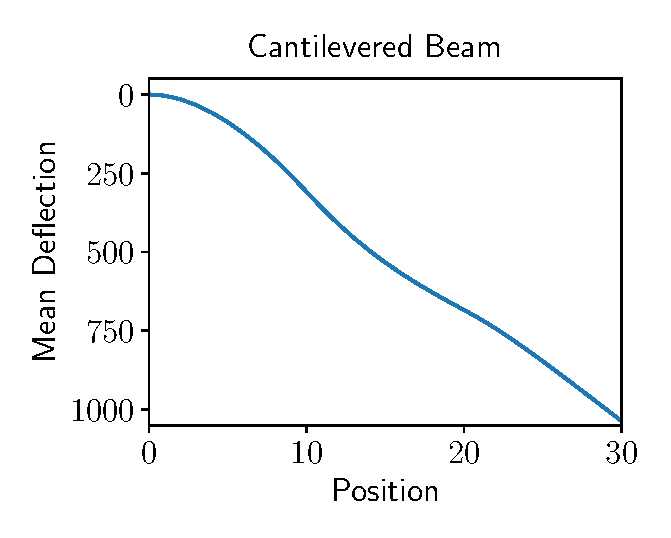
\includegraphics[width=0.33\textwidth]{cantileveredbeamwords.eps}
	\end{tabular}


\end{frame}








%%%%%%%%%%%%%%%%%%%%%%%%%%%%%%%%%%%%%%%%%%
%%%%%%%%%%%%%%%%%%%%%%%%%%%%%%%%%%%%%%%%%%
\section{Beginning}
%%%%%%%%%%%%%%%%%%%%%%%%%%%%%%%%%%%%%%%%%%
%%%%%%%%%%%%%%%%%%%%%%%%%%%%%%%%%%%%%%%%%%
\begin{frame}{Family of Physicists}
	\begin{itemize}
		\item Fred S. Hickernell (father), PhD \alert{Physics}, IEEE Fellow, Motorola researcher
		\item Robert K. Hickernell (brother), PhD \alert{Physics}, NIST Division Director
		\item Thomas S. Hickernell (brother), PhD \alert{Physics}, Motorola researcher, elite charter school teacher
		\item<2> Myself, BA mathematics and physics who became an \alert{applied mathematician}
	\end{itemize}
\end{frame}

\begin{frame}<1-3>[label=summary]{Summary}
\vspace{-3ex}
Problems in Bayesian inference, uncertainty quantification, quantitative finance, (high energy) physics\only<1>{\footfullcite{CouEtal22a,Bla22a,Everett2021,Liyanage2022}}, etc.\ require \alert{numerically} evaluating
\[
\underbrace{\Ex[f(\vX)]}_{\text{expectation}} =  \underbrace{\int_\Omega f(\vx) \, \varrho(\vx) \, \dif \vx}_{\text{integral}}, \qquad \vX \sim \varrho
\]
\only<1>{Other more complicated problems include computing quantiles or marginal distributions.

\vspace{-2ex}}

\vspace{-3ex}
\uncover<2->{There is value in

	\vspace{-2ex}
\begin{itemize}
    \item \alert{low discrepancy} sampling, aka \alert{quasi-Monte Carlo} methods
    \item data-driven \alert{error bounds}
    \item \alert{flattening} and \alert{reducing the effective dimension} of the integrand
    \item quality quasi-Monte Carlo \alert{software} like \hyperlink{https://github.com/QMCSoftware/QMCSoftware}{\alert{qmcpy}\only<2>{\footfullcite{QMCPy2020a}}}
    \item physicists and quasi-Monte Carlo theorists \alert{collaborating} more
\end{itemize}

\only<3>{\addtocounter{footnote}{1}\alert{Caveat:}  I know little about Markov Chain Monte Carlo (MCMC); limited success  combining  with quasi-Monte Carlo\only<3->{\footfullcite{CheDicOwe11a,OweTri05a}.}}}
\only<4>{Slides at \href{https://speakerdeck.com/fjhickernell/argonne2023maytalk}
	{\nolinkurl{speakerdeck.com/fjhickernell/argonne2023maytalk}}

	Jupyter notebook with computations and figures \href{https://github.com/QMCSoftware/QMCSoftware/blob/develop/demos/talk_paper_demos/Argonne_Talk_2022_May/Argonne_2023_Talk_Figures.ipynb}{\beamerbutton{here}}. Visit us at \href{https://qmcpy.org}{\nolinkurl{qmcpy.org}}}
\end{frame}

\section{Trio Identity}

\begin{frame}{Trapezoidal rule}

\vspace{-3ex}
Trio identity \footfullcite{Hic17a,Men16a,CouEtal22a} --- the error of approximating an expectation or integral expressed as the product of \alert{three} quantities

\vspace{-6ex}
\hspace*{-2ex}
\begin{tabular}{m{0.6\textwidth}m{0.4\textwidth}}
    \begin{multline*}\int_0^1 f(x) \, \dif x - \sum_{i=0}^n w_i f(x_i)
    \alert{=0.112} \qquad w_i = \frac{x_{i+1} - x_{i-1}}{2}\\
    = \underbrace{\frac{\int_0^1 f(x) \, \dif x - \sum_{i=0}^n w_i f(x_i)}{\frac{\max_{i}(x_{i+1} - x_i)^2}{8} \,
    \int_0^1 \abs{f''(x)} \, \dif x}}_{\alert{\substack{\text{misfortune} \\ 0.151 \\\uncover<2->{\text{\normalsize confounding}}}}}
    \, \underbrace{\frac{\max_{i}(x_{i+1} - x_i)^2}{8}}_
    {\alert{\substack{\text{sampling deficit}\\ 0.020 \\\uncover<2->{\text{\normalsize discrepancy}}}}} \,
    \underbrace{\int_0^1 \abs{f''(x)} \, \dif x}_{\alert{\substack{\text{roughness} \\ 37.3\\
    \uncover<2->{\text{\normalsize variation}}}}}
    \end{multline*}
    \uncover<2->{
    \vspace{-2.5ex}
    \begin{itemize}
    \item Confounding is \alert{between $-1$ and $1$} {\scriptsize \parencite[(7.15)]{BraPet11a}}
    \item Discrepancy \only<2>{depends upon \alert{sample} only}\only<3->{reduced via \alert{clever} or more sampling}
    \item Variation \only<2>{depends on \alert{integrand} only, semi-norm}\only<3->{value unknown, reduced via \alert{transformations}}
\end{itemize}}
    & 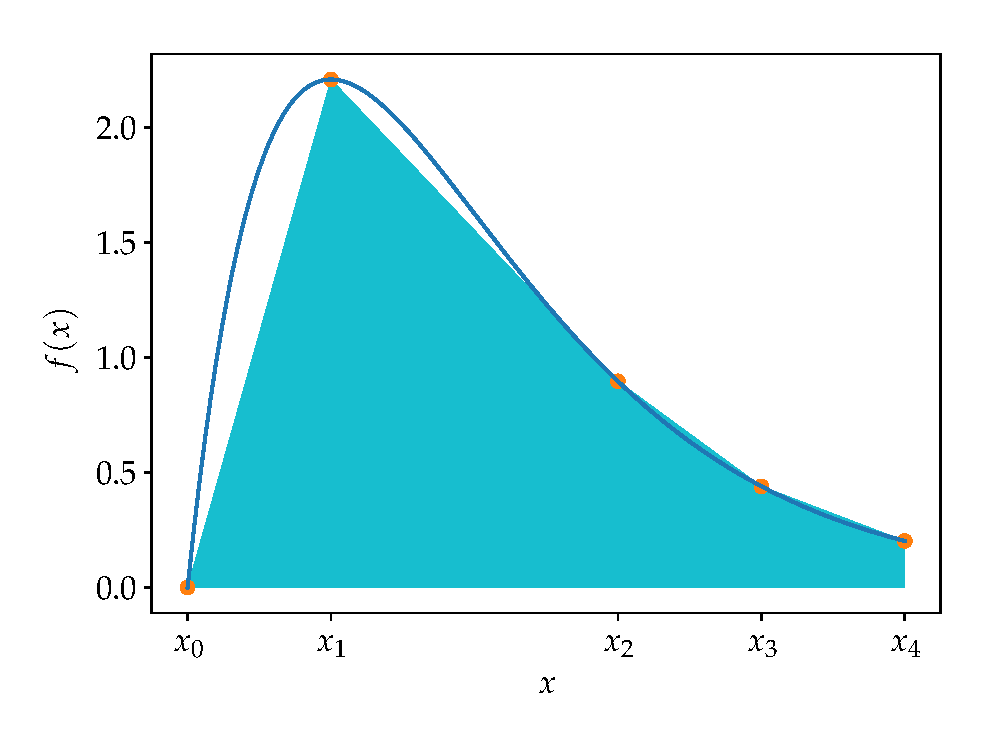
\includegraphics[width=0.4\textwidth]{traprule.eps}
\end{tabular}
\vspace{-2ex}

\end{frame}

\begin{frame}{Independent and Identically Distributed (IID) Monte Carlo}

	\vspace{-6ex}
	\hspace*{-2ex}
	\begin{tabular}{m{0.65\textwidth}m{0.35\textwidth}}
		\begin{multline*}\overbrace{\int_{\reals^d} f(\vx) \, \varrho(\vx) \, \dif \vx}^{\Ex[f(\vX)],\ \vX \sim \varrho} - \frac 1n \sum_{i=0}^n f(\vx_i) \hspace{6ex} \vx_i \IIDsim \varrho
			\\
			= \underbrace{\frac{\int_{\reals^d} f(x) \, \varrho(\vx) \, \dif \vx - \frac 1n \sum_{i=0}^n f(\vx_i)}{\frac 1{\sqrt{n}} \,
					\std[f(\vX)]}}_{\alert{\text{confounding}}}
			\, \underbrace{\frac{1}{\sqrt{n}}}_
			{\alert{\text{discrepancy}}} \,
			\underbrace{\std(f(\vX))}_{\alert{\text{variation}}}
		\end{multline*}
			\vspace{-2.5ex}
			\begin{itemize}
				\item $\RMS[\text{confounding}] = 1$, but confounding could be $\Order(\sqrt{n})$
				\item Discrepancy depends on sample size only
				\item Variation reduced through transformations
		\end{itemize}
		&
		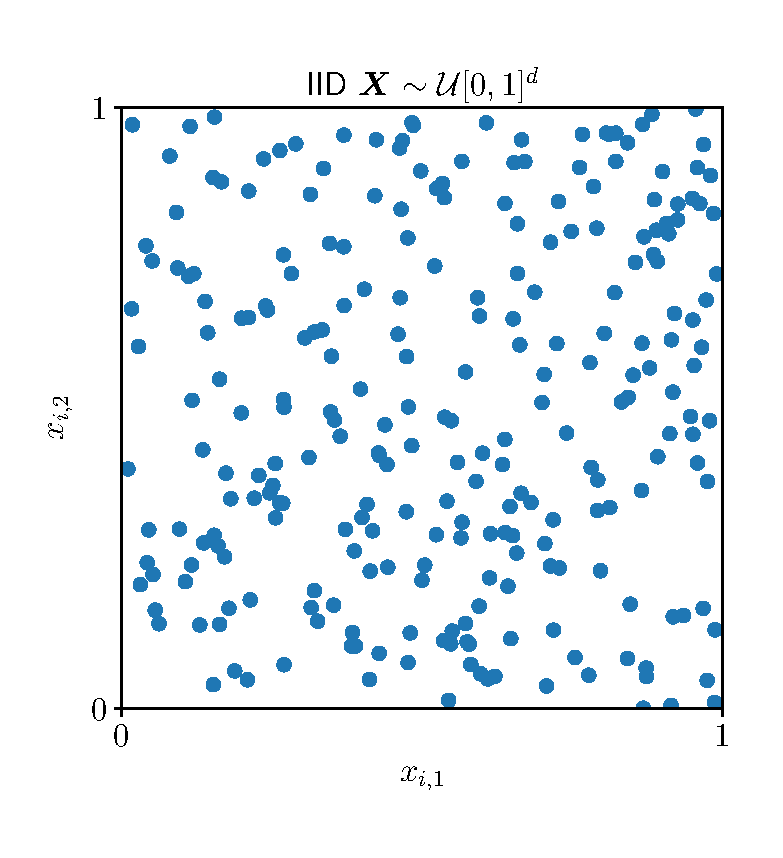
\includegraphics[width=0.35\textwidth]{iidptssingle.eps}
	\end{tabular}
	\vspace{-2ex}

\end{frame}


\begin{frame}{Low Discrepancy Sampling aka  Quasi-Monte Carlo\footfullcite{Hic97a}}

	\vspace{-5ex}
	\hspace*{-2ex}
	\begin{tabular}{m{0.65\textwidth}m{0.35\textwidth}}
		\vspace{-4ex}
		\[
        \begin{aligned}
		    \MoveEqLeft{\overbrace{\int_{[0,1]^d} f(\vx) \, \dif \vx}^
            {\Ex[f(\vX)], \ \vX \sim \cu[0,1]^d} - \frac 1n \sum_{i=0}^n f(\vx_i)
			= \CONF(f,\{\vx\}_{i=1}^n) \, \DISC(\{\vx\}_{i=1}^n) \, \VAR(f)} \\
        \only<6>{ \MoveEqLeft{\CONF(f,\{\vx_i\}_{i=1}^n) = \frac{\int_{[0,1]^d} f(\vx) \, \dif \vx - \frac 1n \sum_{i=0}^n f(\vx_i)}{\DISC(\{\vx_i\}_{i=1}^n) \, \VAR(f)}   \quad \text{between } \pm1}}
         \only<2-5>{\MoveEqLeft{\DISC^2(\{\vx_i\}_{i=1}^n) = \left(\frac{13}{12}\right)^2} \\
         &
         - \frac 2n \sum_{i=1}^n \prod_{j=1}^d\left(1 + 0.5\abs{x_{ij} - 0.5} - 0.5(x_{ij}-0.5)^2\right) \\
         & + \frac{1}{n^2} \sum_{i,k=1}^n \left[ 1 + 0.5\abs{x_{ij} - 0.5} +
         0.5\abs{x_{kj} - 0.5} - 0.5\abs{x_{ij} - x_{kj}}\right]}
         \only<1>{\MoveEqLeft{\VAR^2(f)
          = \int_{[0,1]} \left[\frac{\partial f}{\partial x_1} (x_1, 0.5, \ldots, 0.5)\right]^2 \, \dif x_1 + \cdots }\\
         & + \int_{[0,1]^{2}} \left[\frac{\partial^2 f}{\partial x_1 \partial x_2} (x_1, x_2,0.5, \ldots, 0.5)\right]^2 \, \dif x_1 \, \dif x_2 + \cdots \\
         & + \int_{[0,1]^{d}} \left[\frac{\partial^d f}{\partial x_1 \cdots \partial x_d} (\vx)\right]^2 \, \dif \vx
         }
		\end{aligned}
        \]
		&
		\centering
		\only<1-2,6>{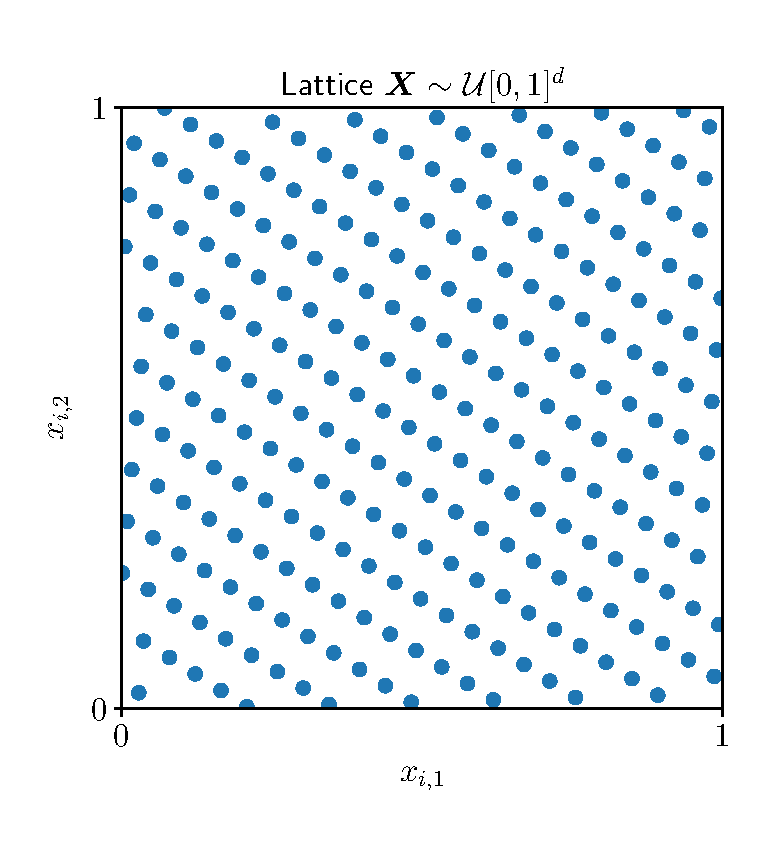
\includegraphics[width=0.35\textwidth]{latticeptssingle.eps}}
		\only<3>{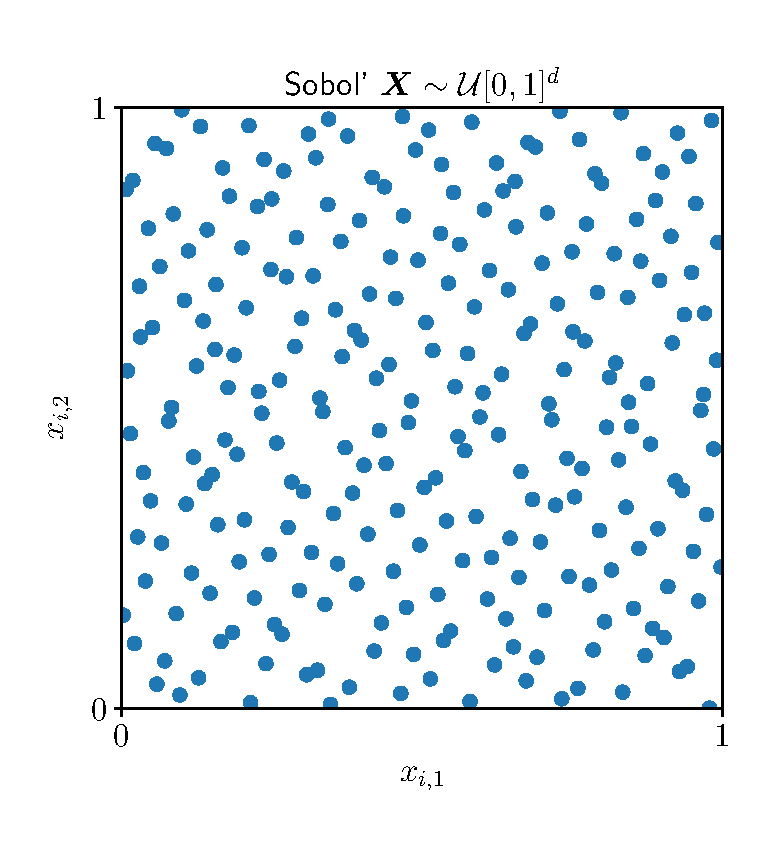
\includegraphics[width=0.35\textwidth]{sobolptssingle.eps}}
		\only<4>{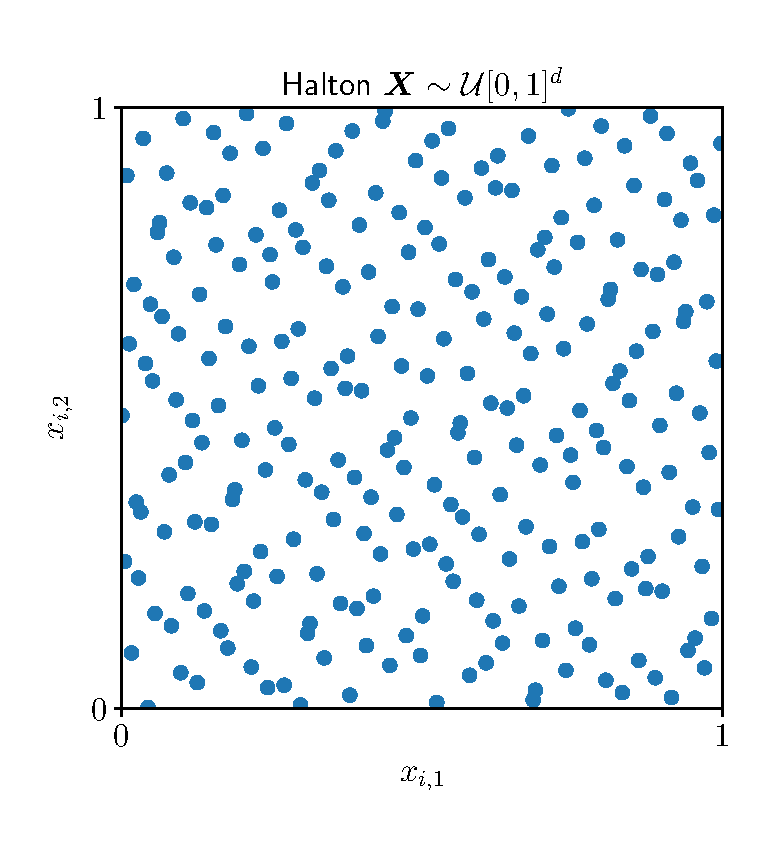
\includegraphics[width=0.35\textwidth]{haltonptssingle.eps}}
		\only<5>{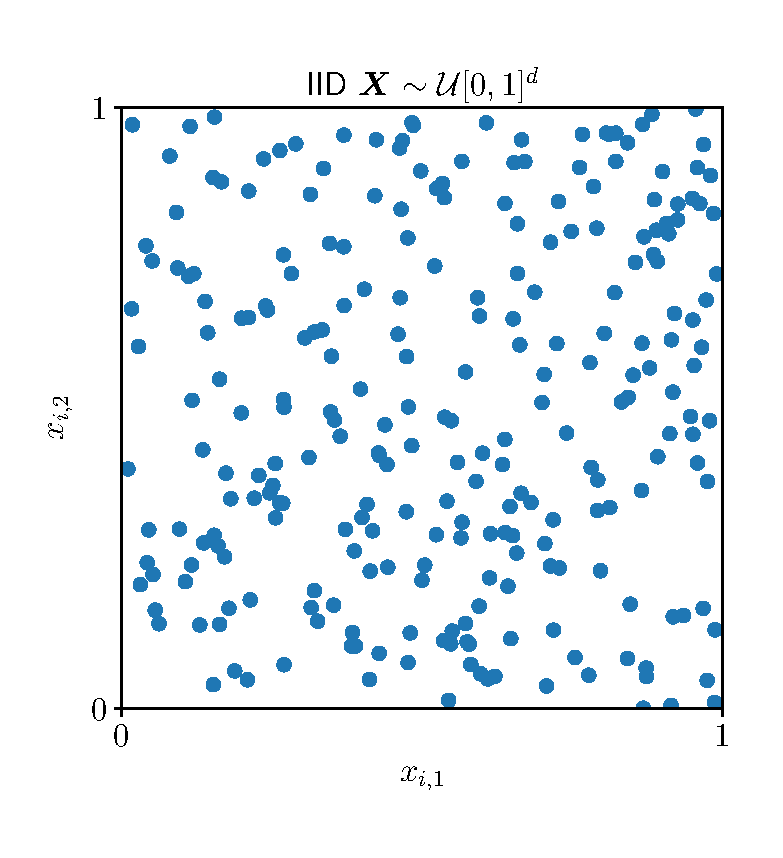
\includegraphics[width=0.35\textwidth]{iidptssingle.eps}}
		\only<2-4,6>{\vspace{-4ex}
		\[\DISC(\{\vx_i\}_{i=1}^n) = \alert{\Order(n^{-1+\delta})}\]}
		\only<5>{\vspace{-4ex}
	\[\DISC(\{\vx_i\}_{i=1}^n) = \alert{\Order(n^{-1/2})}\]}
	\end{tabular}
	\vspace{-5ex}

        \only<1>{$\VAR$ is a semi-norm, more smoothness than $\std$, value generally unknown, reduced through transformations}%
        \only<2>{\vspace{-1ex} $\DISC$ is the norm of the error functional, value known with $\Order(dn^2)$ operations}

\end{frame}


\begin{frame}{Uncertainty in a Cantilevered Beam\footfullcite{ParSee22a}}
	\vspace{-4ex}
	\begin{tabular}{m{0.6\textwidth}m{0.4\textwidth}}
		\[
		\begin{aligned}
			u(x) & = g(\vZ, x) = \text{beam deflection} \\
			& = \text{solution of a differential equation boundary value problem} \\
			\vZ & \sim \cu[1,1.2]^3 \quad \text{defines uncertainty in Young's modulus} \\
			x &= \text{position} \\
			\mu(x) &= \Ex[g(\vZ,x)] = \int_{[0,1]^3}  g(\vz,x) \, \dif \vz \approx \frac 1n \sum_{i=1}^n g(\vZ_i,x)
			\\
			& \mu(\text{end}) = 1037
		\end{aligned}
		\]
		&
		\centering
		\vspace{1.5ex}
		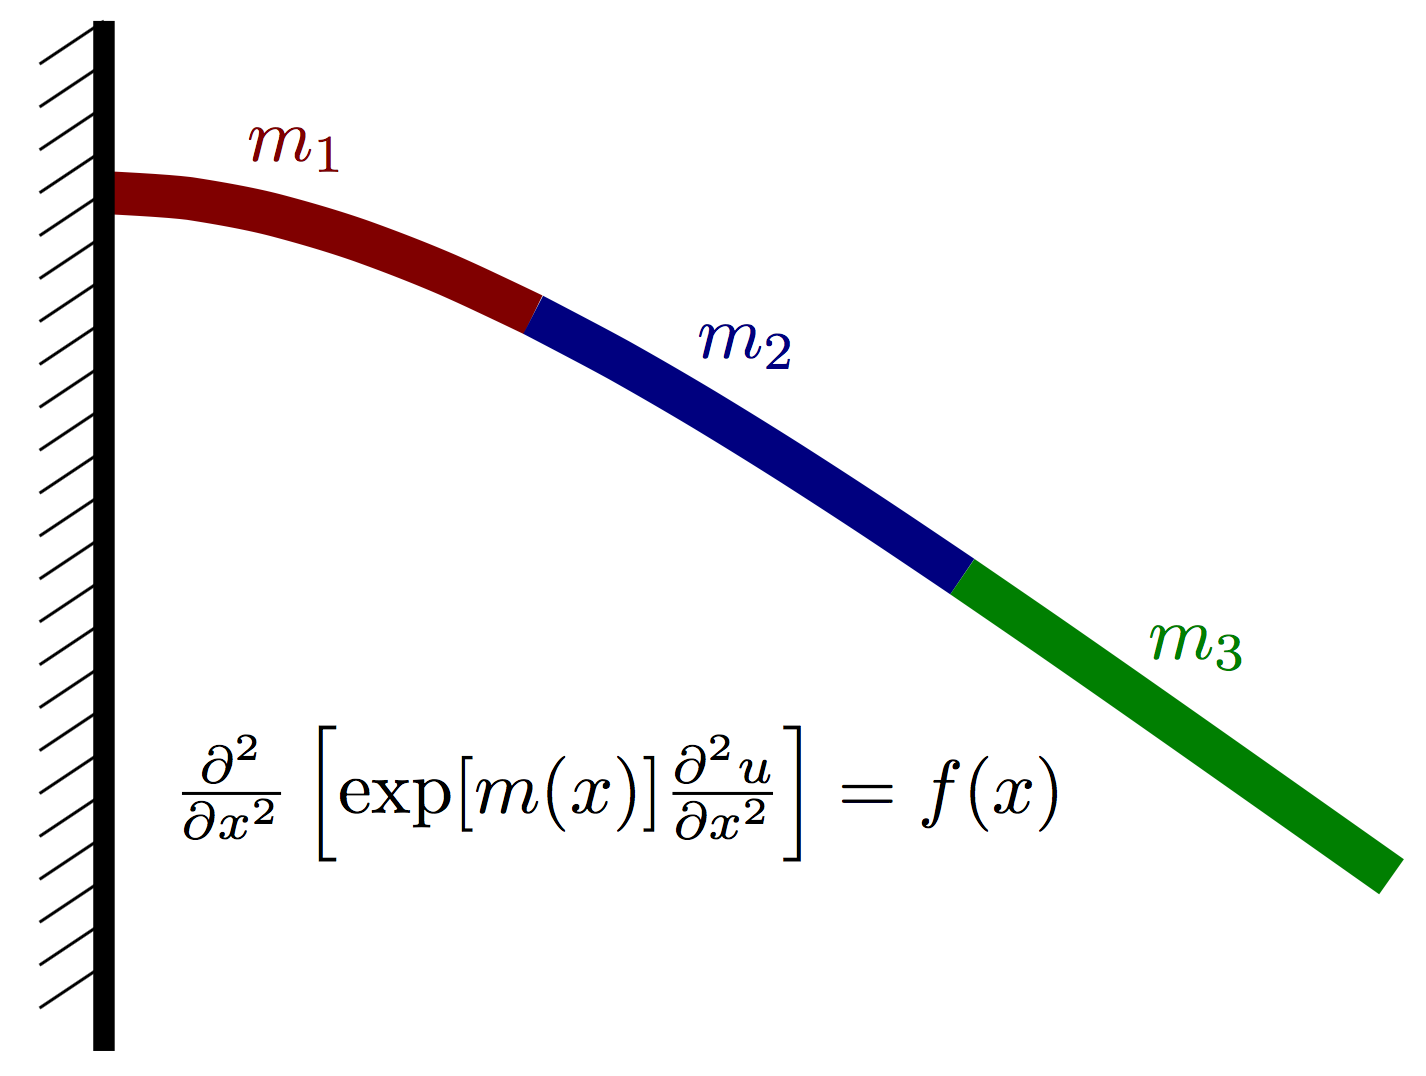
\includegraphics[width=0.35\textwidth]{BeamDrawing.png} \newline
	\end{tabular}


\end{frame}

\begin{frame}{IID vs.\ Low Discrepancy for the Cantilevered Beam via QMCPy\footfullcite{QMCPy2020a}}
	\vspace{-2ex}
	\begin{tabular}{m{0.63\textwidth}m{0.35\textwidth}}
		\vspace*{-10ex}
		\[
		\begin{aligned}
				g(\vZ, x) &= \text{beam deflection} \\
			\only<1>{\vZ & \sim \cu[1,1.2]^3 \quad \text{defines uncertainty} \\
			x &= \text{position} \\}
			\mu(x) &= \Ex[g(\vZ, x)] &
			\mu(\text{end}) &= 1037
		\end{aligned}
		\]
		&
		\centering
		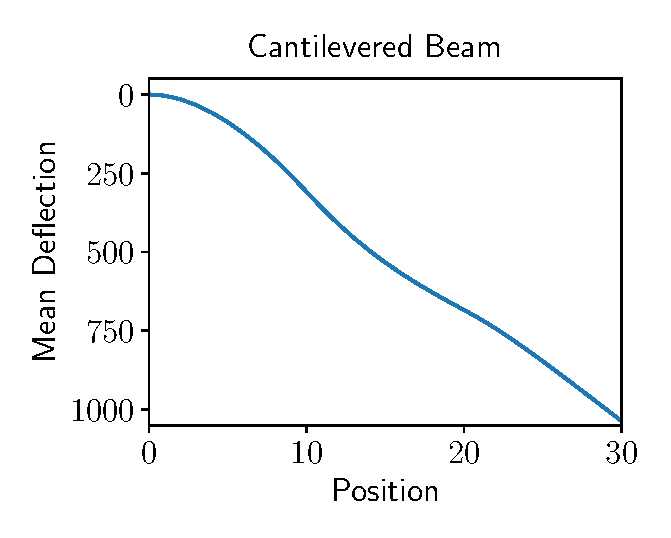
\includegraphics[width=0.33\textwidth]{cantileveredbeamwords.eps}
	\end{tabular}

	\vspace{-11ex}\only<2>{\vspace{-3ex}}
	\includegraphics<1>[width=0.6\textwidth]{iidldbeam.eps}
	\includegraphics<2>[width=0.65\textwidth]{ldparallelbeam.eps}

\end{frame}

\begin{frame}{Low Discrepancy Points Fill Space}
\vspace{-3.2ex}

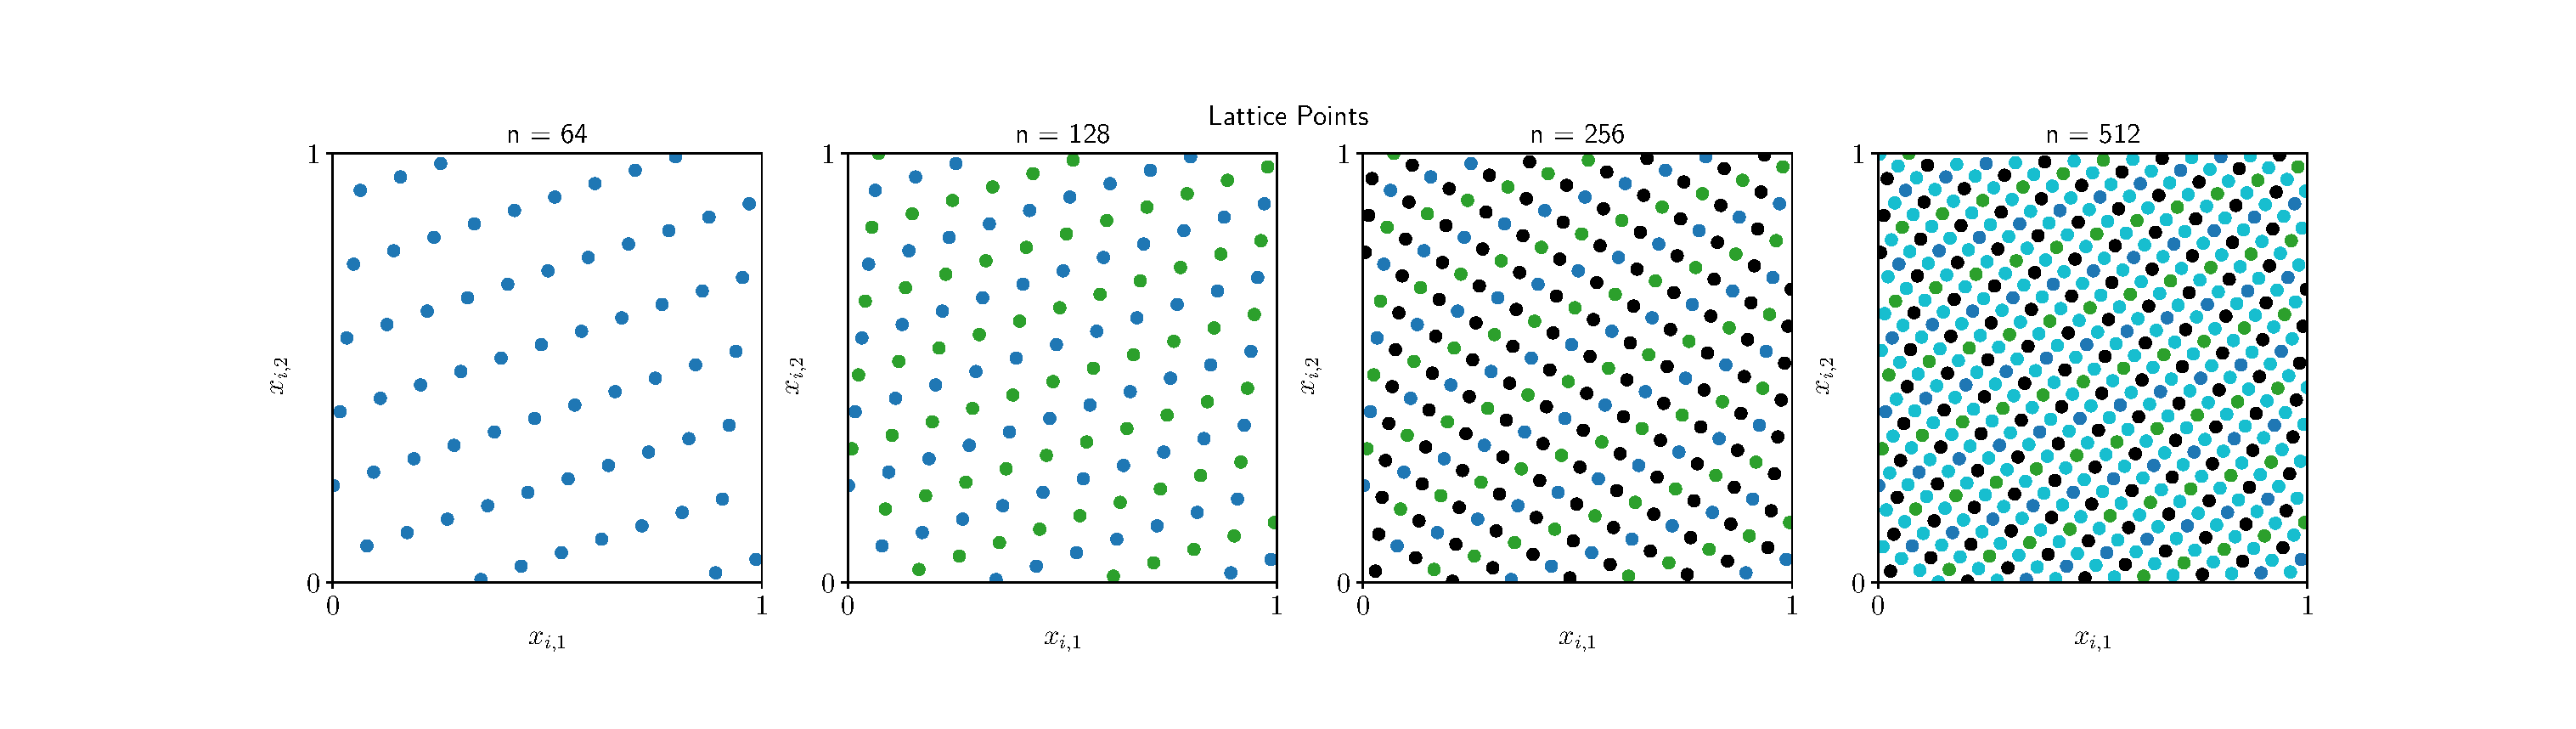
\includegraphics[width=\textwidth]{latticeptsseq.eps}

\vspace{-4.3ex}

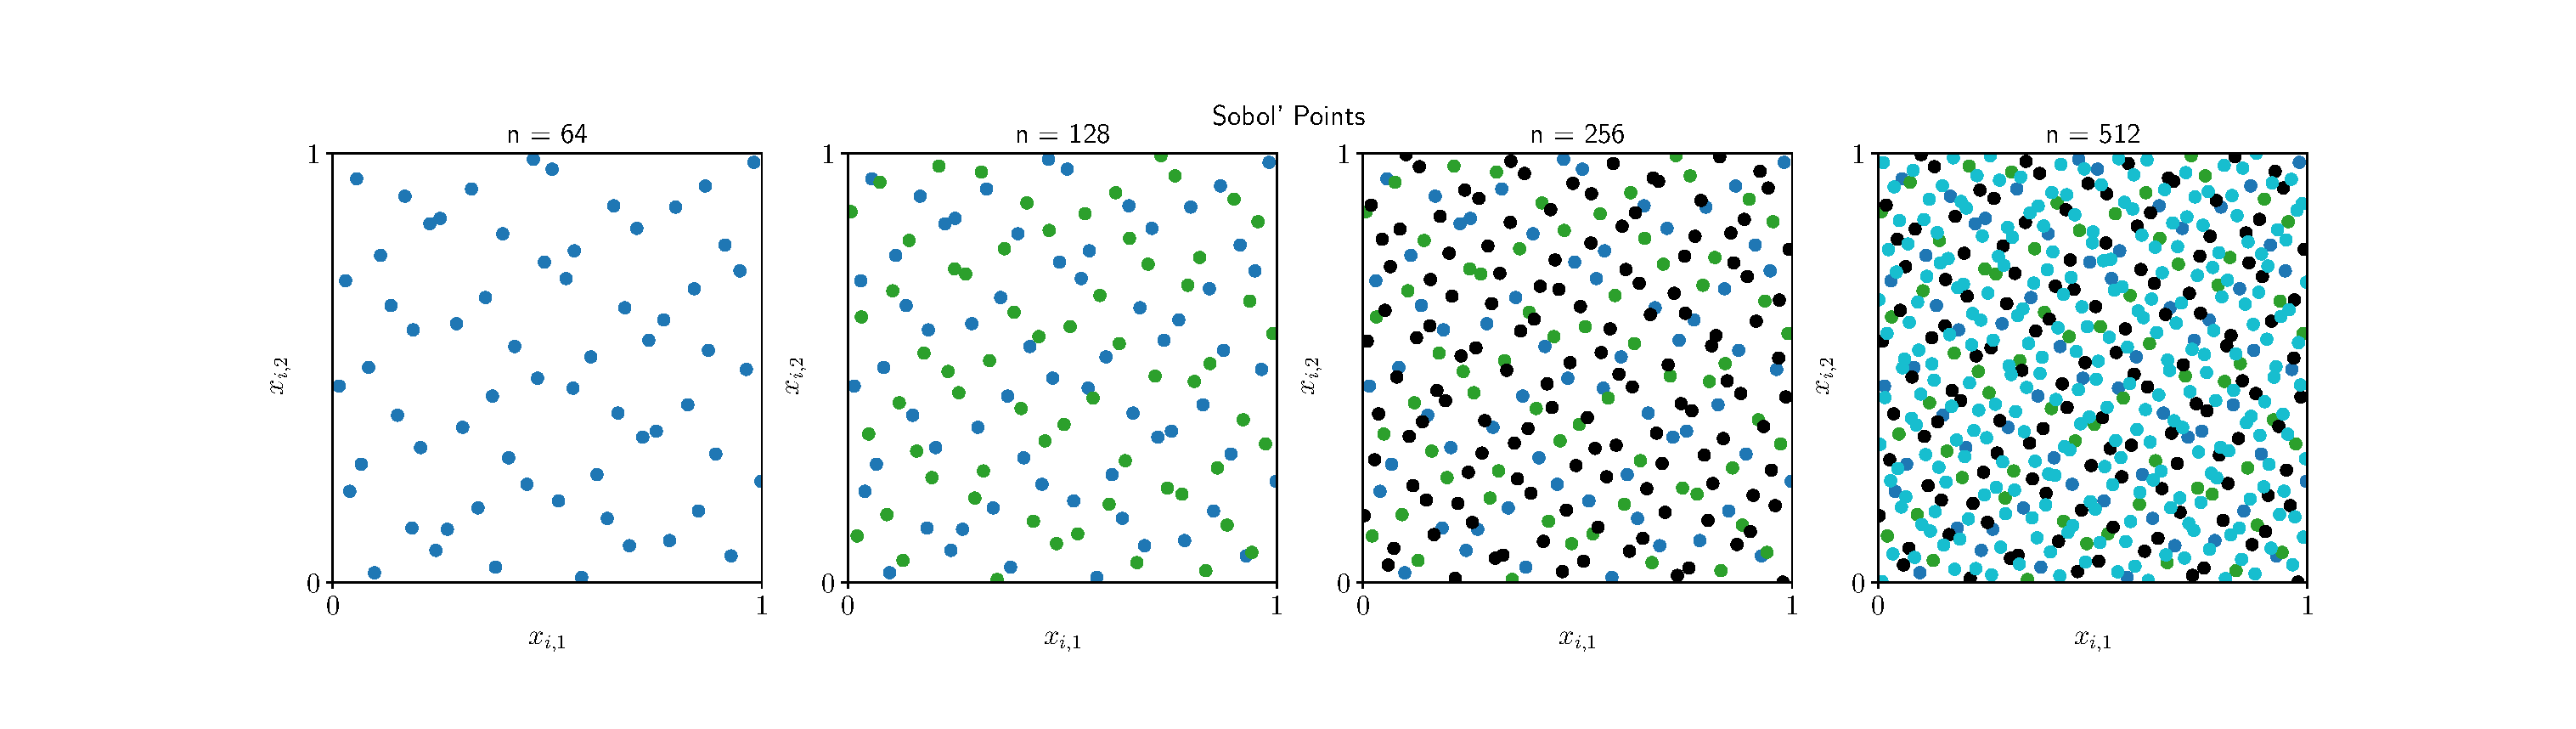
\includegraphics[width=\textwidth]{sobolptsseq.eps}

\end{frame}

\begin{frame}{Low Discrepancy Points Look ``Good'' in All Coordinate Projections}
	\vspace{-3.2ex}

	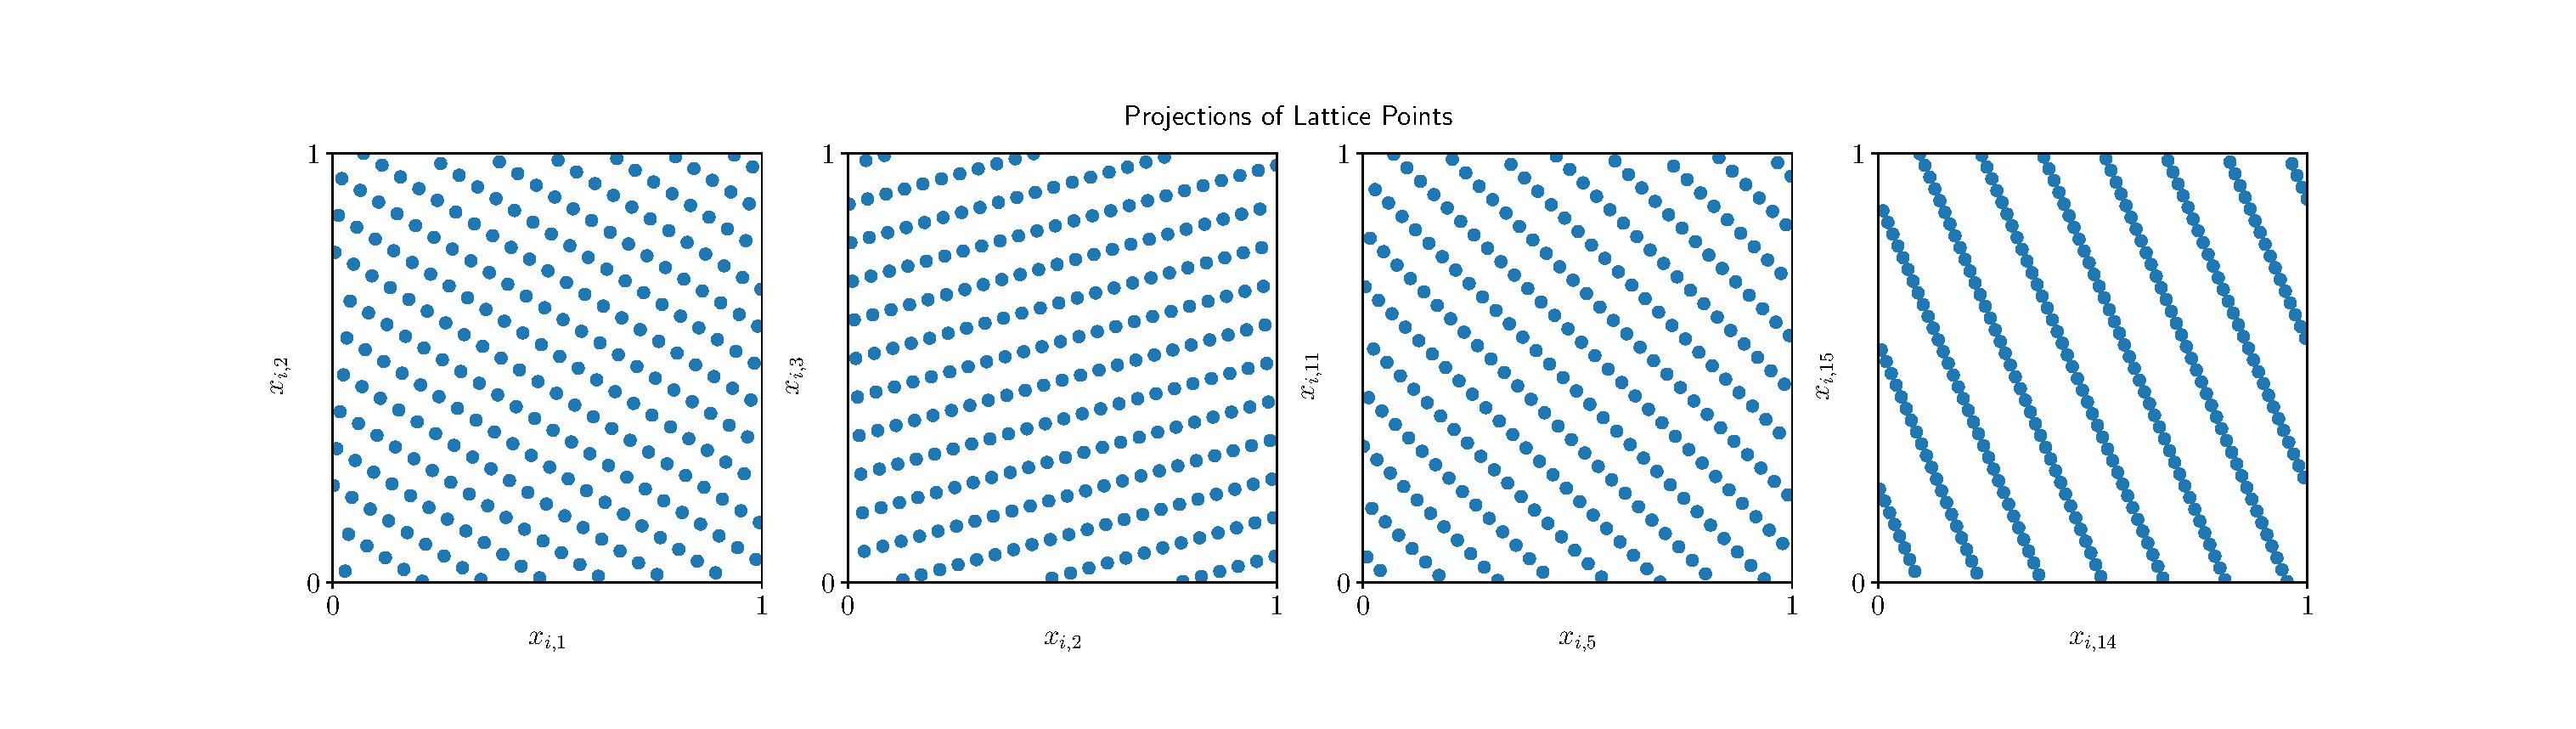
\includegraphics[width=\textwidth]{latticeptsproj.eps}

	\vspace{-4.3ex}

	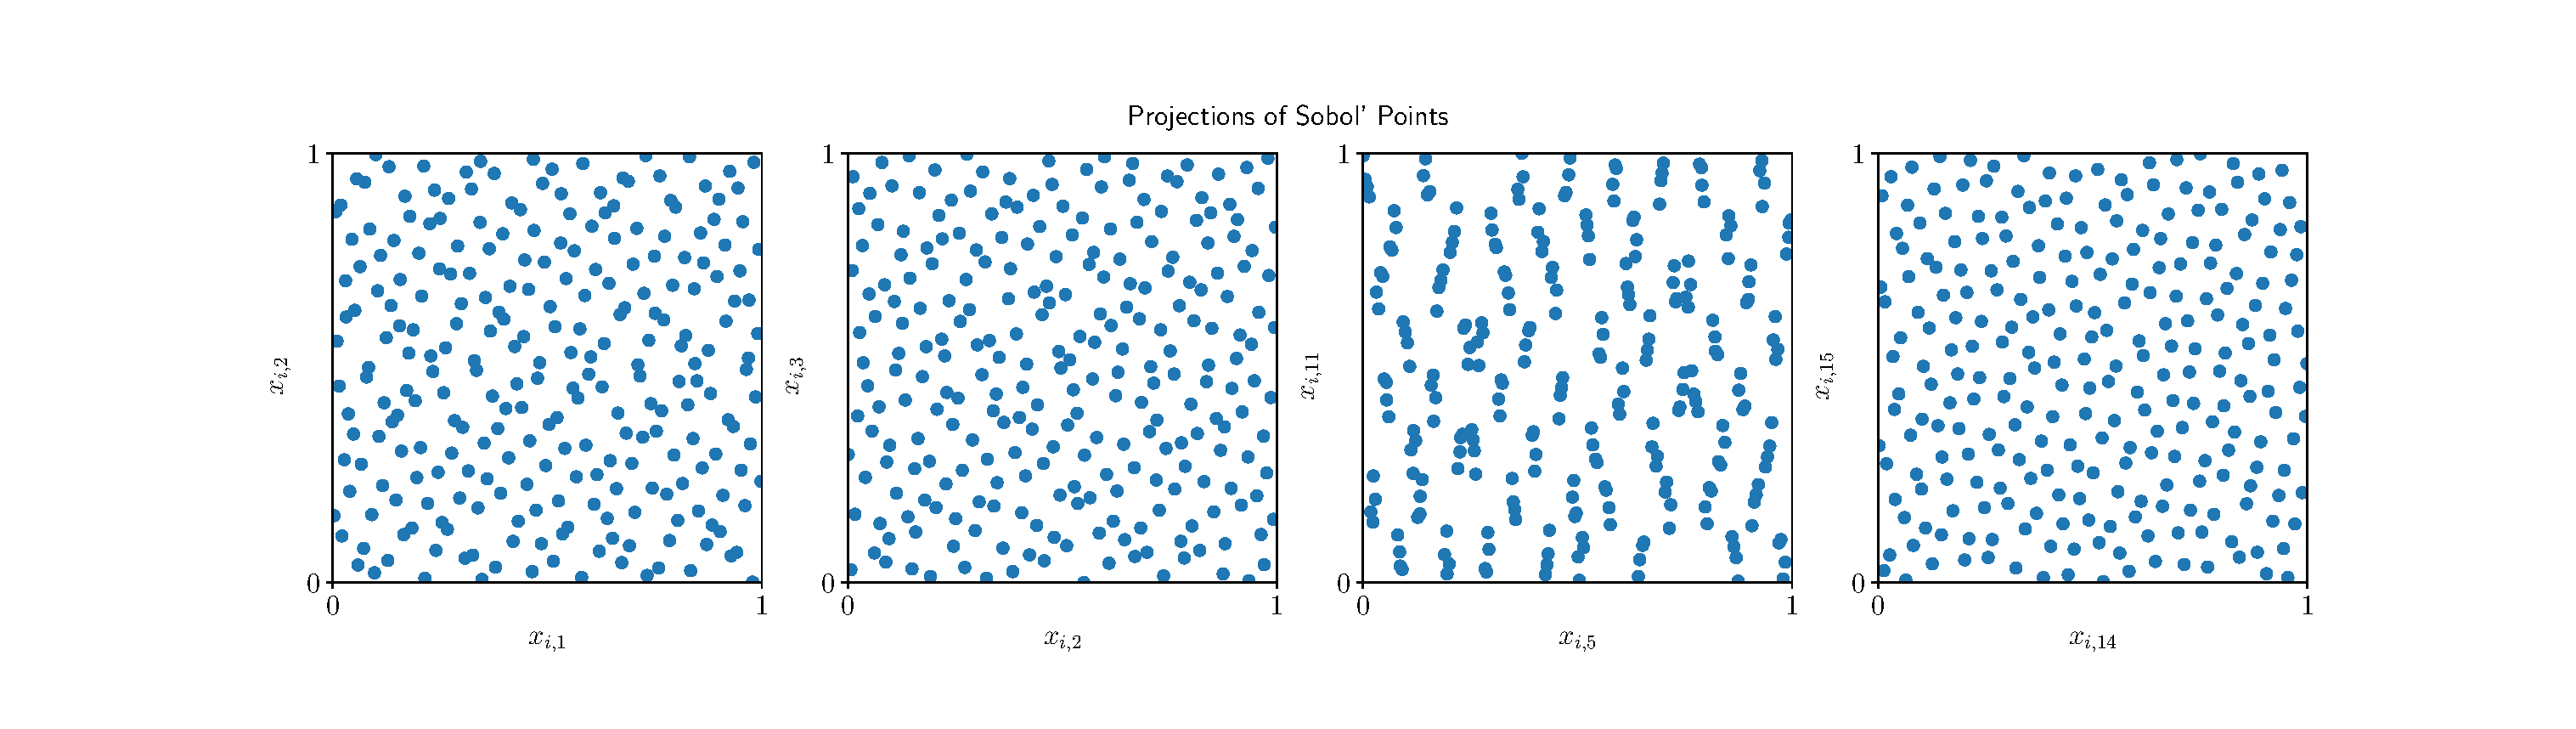
\includegraphics[width=\textwidth]{sobolptsproj.eps}


\end{frame}

\begin{frame}{Low Discrepancy Points Can Be Randomized}
	\vspace{-3.2ex}

	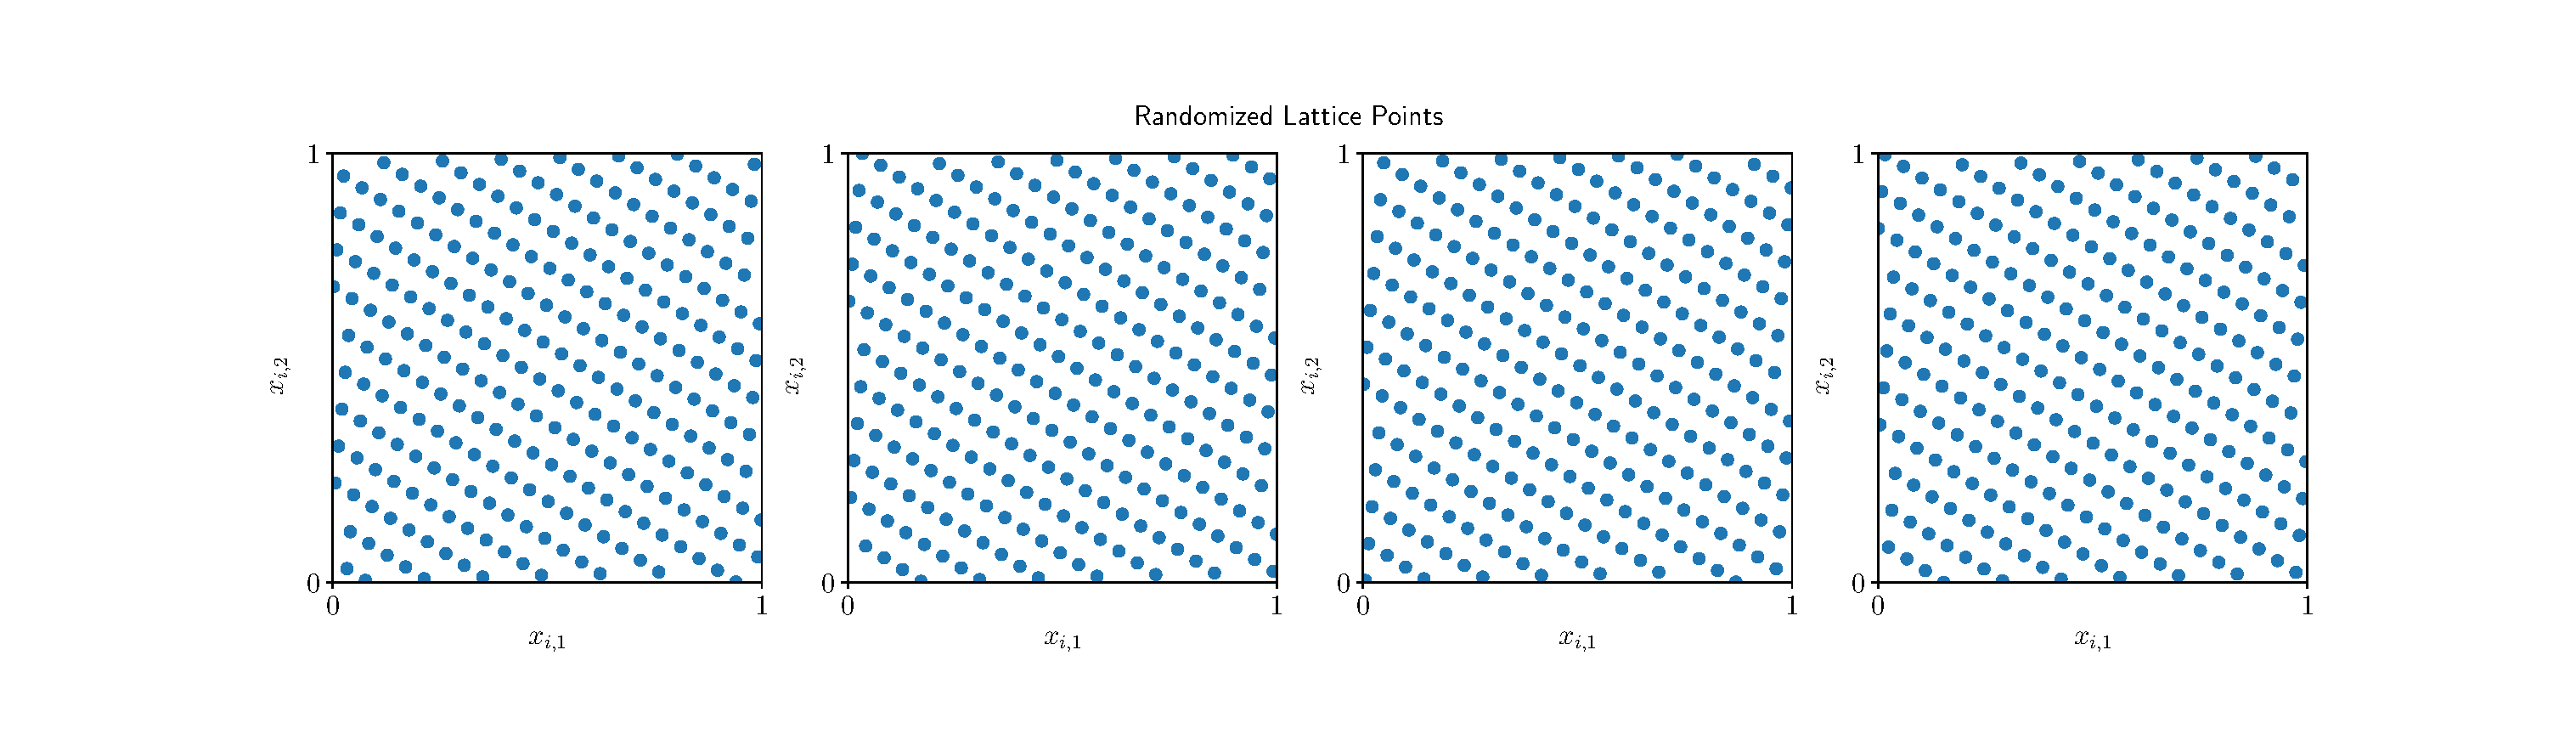
\includegraphics[width=\textwidth]{latticeptsrand.eps}

	\vspace{-4.3ex}

	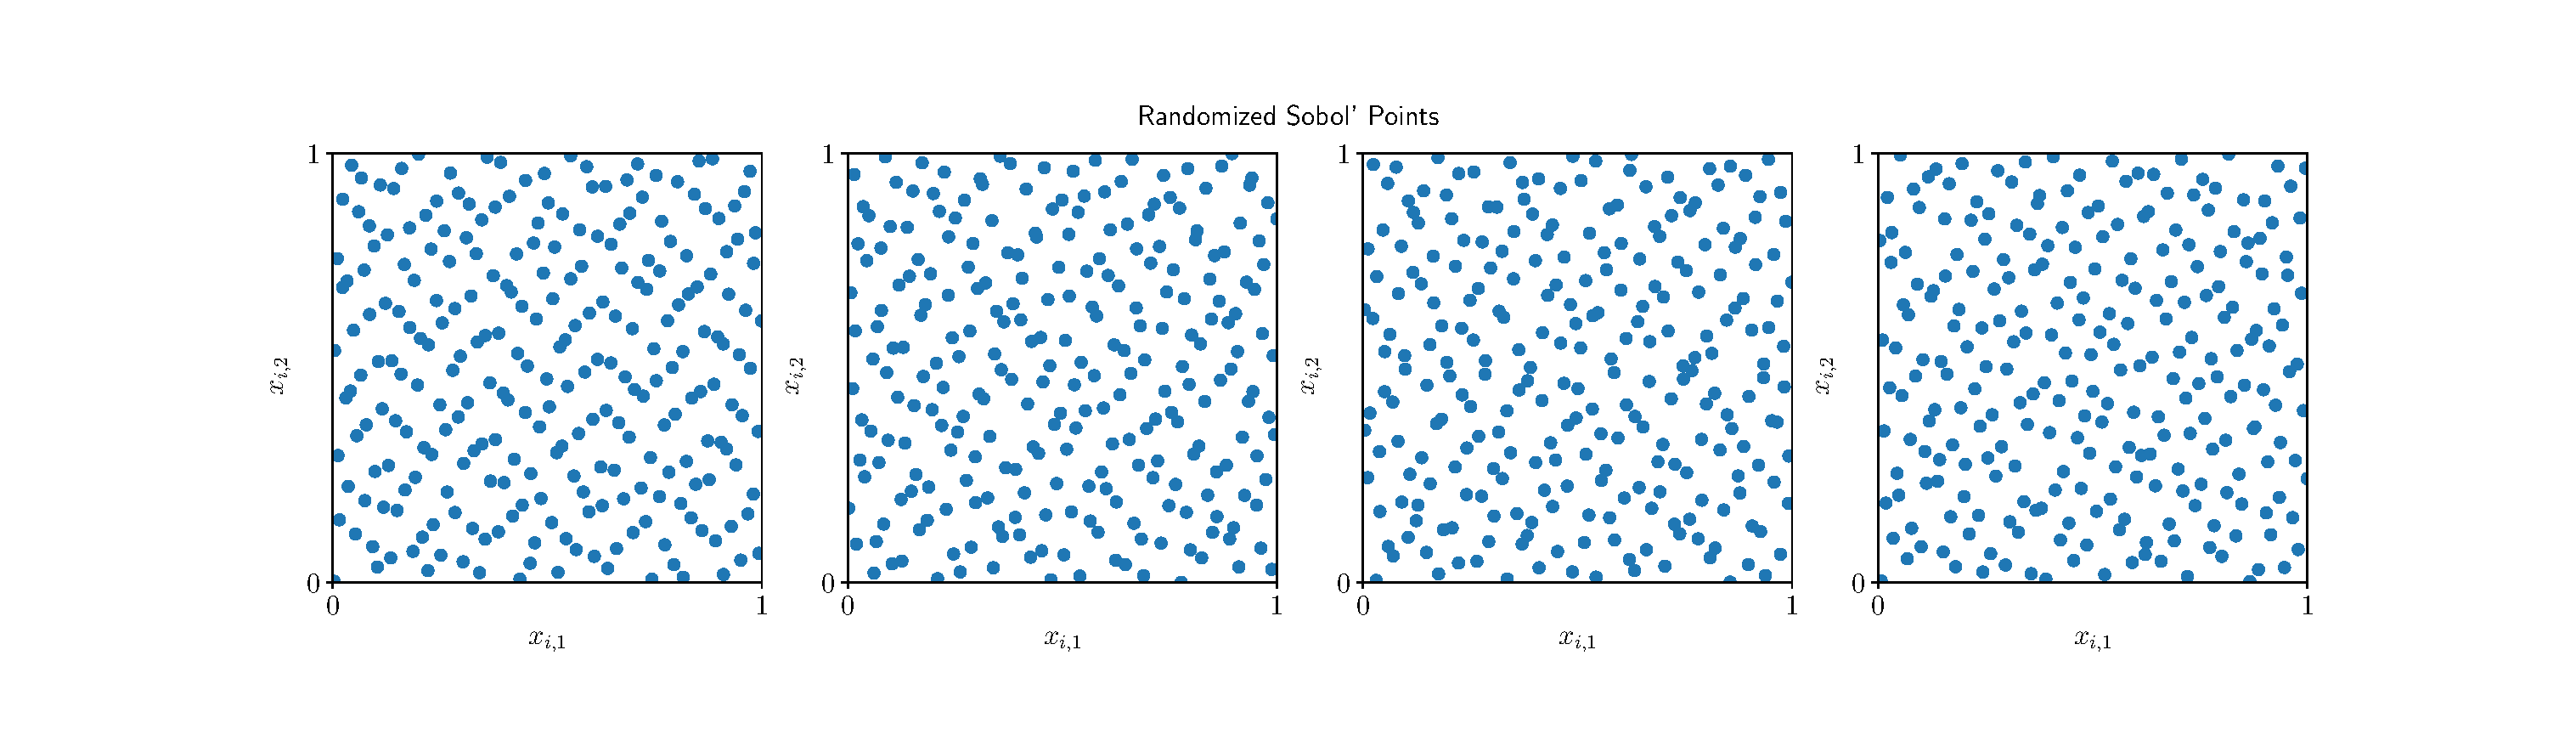
\includegraphics[width=\textwidth]{sobolptsrand.eps}


\end{frame}

\begin{frame}{Lessons from the Trio Identity}
	\vspace{-8ex}
	\[
	\overbrace{\int_{[0,1]^d} f(\vx) \, \dif \vx}^
				{\Ex[f(\vX)], \ \vX \sim \cu[0,1]^d} - \frac 1n \sum_{i=0}^n f(\vx_i)
				= \CONF(f,\{\vx\}_{i=1}^n) \, \DISC(\{\vx\}_{i=1}^n) \, \VAR(f)
	\]

\vspace{-2ex}
\begin{itemize}
	\item Use \alert{low discrepancy}\footfullcite{DicPil10a,DicEtal14a,DicEtal22a} instead of IID sampling for performance gains
	\item<2-> \alert{Randomize} when possible so avoid bad $\CONF(f,\{\vx\}_{i=1}^n)$. \only<3->{Scrambled Sobol' often beats unscrambled Sobol' in order of convergence.  Randomizing moves points off the boundaries.}
	\item<3-> Error decay rate, $\DISC(\{\vx\}_{i=1}^n)$, \alert{limited} by the assumptions on $f$ implicit in the choice of $\VAR$
	\item<3-> \alert{Deterministic} trio identities constrain $-1 \le \CONF(f,\{\vx\}_{i=1}^n) \le 1$ but  may be \alert{pessimistic}
	\item<3-> If $\CONF(f,\{\vx\}_{i=1}^n)$ is consistently small, look for a \alert{better choice} of $\VAR$ and $\DISC$
	\item<4-> \alert{Theory} explains how well an algorithm works; practice can help sharpen theory
\end{itemize}

\end{frame}


\section{Stopping Rules}
\begin{frame}{Estimating or Bounding the Error from Simulation Data}
	\vspace{-10ex}
\only<1-2>{	\[
	\overbrace{\int_{[0,1]^d} f(\vx) \, \dif \vx}^
	{\Ex[f(\vX)], \ \vX \sim \cu[0,1]^d} - \frac 1n \sum_{i=0}^n f(\vx_i)
	= \CONF(f,\{\vx\}_{i=1}^n) \, \DISC(\{\vx\}_{i=1}^n) \, \VAR(f)
	\]
When to \alert{stop} sampling because the error is small enough?

\vspace{-2ex}
\begin{itemize}
	\item $\VAR(f)$ is \alert{impractical} to bound
	\item $\DISC(\{\vx\}_{i=1}^n)$ is \alert{expensive} to calculate
\end{itemize}

\vspace{-1ex}
\only<2>{Many do replications

\vspace{-4ex}
\[
\Biggl \lvert \int_{[0,1]^d} f(\vx) \, \dif \vx - \frac 1n \sum_{i=0}^n f(\vx_i) \Biggr \rvert^2
\approx \frac{\alert{\text{fudge}^2}}{R} \sum_{r=1}^R \left(\frac 1{Rn} \sum_{q,i=1}^{R,n} f(\vx^{(q)}_{i}) - \frac 1n \sum_{i=1}^n  f(\vx^{(r)}_{i}) \right)^2
\]
where $\{\vx^{(1)}_i\}_{i=1}^n, \ldots \{\vx^{(R)}_i\}_{i=1}^n$ are randomizations of a low discrepancy sequence.}}

\only<3>{\vspace{6ex}
	For $\begin{Bmatrix} \text{lattice} \\ \text{Sobol'}\end{Bmatrix}$  or  sampling

	\vspace{-2ex}
\[
\Biggl\lvert \int_{[0,1]^d} f(\vx) \, \dif \vx - \frac 1n \sum_{i=0}^n f(\vx_i) \Biggr \rvert \le \sum_{\vk \in \text{dual lattice}} \bigl\lvert\hf(\vk) \bigr\rvert
\]
where $\hf(\vk)$ are the Fourier $\begin{Bmatrix} \text{complex exponential} \\ \text{Walsh}\end{Bmatrix}$ coefficients of $f$ and the \alert{dual lattice} consists of wave numbers of $\begin{Bmatrix} \text{complex exponential} \\ \text{Walsh}\end{Bmatrix}$ bases that are perfectly aliased with $1$.

Rigorous data-driven error bounds  based on sums of discrete Fourier $\begin{Bmatrix} \text{complex exponential} \\ \text{Walsh}\end{Bmatrix}$ coefficients of $f$ are valid for not too noisy/peaky $f$\footfullcite{HicJim16a,JimHic16a}.}

\only<4>{Data-driven error bounds based on credible intervals assume that $f$ is an instance of a \alert{Gaussian process} whose parameters are tuned;  valid for $f$ that are not outliers.  Computation is fast if \alert{covariance kernel} matches the sample \footfullcite{RatHic19a,JagHic22a}.}

\end{frame}

\begin{frame}{Problems Involving Several Integrals}

	\vspace{-10ex}
\begin{gather*}
	\text{posterior mean}_j =
	\frac{  \int_{\reals^d} x_j \, \text{likelihood}(\vx,\text{data}) \, \text{prior}(\vx) \, \dif  \vx}
	{ \int_{\reals^d} \text{likelihood}(\vx,\text{data}) \, \text{prior}(\vx) \, \dif  \vx}
	, \qquad j =1, \ldots, d \\
	\text{expected output}(\vs)  = \Ex[\text{output}(\vs,\vX)] =  \int_{\reals^d} \text{output}(\vs,\vx) \, \varrho(\vx) \, \dif \vx , \qquad \vs \in \Omega\\
	\text{sensitivity index}_j = \int_{[0,1]^{2d}} f(\vx)[f(x_j,\vz_{-j}) - f(\vz)] \, \dif \vx \,\dif \vz, \qquad j =1, \ldots, d
\end{gather*}
Stopping criteria have been extended to these cases\footfullcite{HicEtal17a,JagSor23a}
\end{frame}

%\end{document}

\begin{frame}{Bayesian Logistic Regression for Cancer Survival Data}

	\vspace{-10ex}
	\[
	\text{logit}(\text{probability of $5$ year survival}) = \beta_0 + \beta_1 \text{patient age} + \beta_2 \text{operation year} + \beta_3 \text{\# positive axillary nodes}
	\]
	Logistic regression to estimate $\beta_j$ from 306 data\footfullcite{haberman1976generalized} with error criterion of
	\[
	\text{absolute error} \le 0.05 \text{ \& } \text{relative error} \le 0.5
	\]
	\[
	\begin{array}{cccccccc}
		\text{method} & \beta_0 & \beta_1 & \beta_2  & \beta_3
		& \frac{\text{all true}}{\text{all}} & \frac{\text{true pos}}{\text{all pos}} & \frac{\text{true pos}}{\text{true pos $+$ false neg}} \\
		\toprule
		\text{Bayesian \& qmcpy} & 0.0080 & -0.0041 & 0.1299 & -0.1569 & 74\% & 74\% & 100\%\\
		\text{elastic net} & 0.0020 & -0.0120 &  0.0342 &  -0.11478 &  74\% & 77\% & 93\%\\
	\end{array}
	\]
\end{frame}

\begin{frame}{Lessons from Data-Based Error Bounds}

	\vspace{-8ex}
	\[
	\Biggl\lvert\int_{[0,1]^d} f(\vx) \, \dif \vx - \frac 1n \sum_{i=0}^n f(\vx_i) \Bigg \rvert
	\le \text{some function of }\{(\vx_i,f(\vx_i))\}_{i=1}^n
	\]

	\begin{itemize}
		\item Theoretical bounds are \alert{impractical}
		\item Every data-based error bound can be \alert{fooled}
		\item There are \alert{better} choices than random replications
	\end{itemize}
	\bigskip

	\centerline{{\Large $f \in$} \hugecone {\Large not } \largescoop}

\end{frame}

\section{Transforming the Integrand}

\begin{frame}{Importance Sampling and Control Variates}
	\vspace{-5ex}
	The original problem may look like $\int_\Omega g(\vt) \, \dif \vt$.  \uncover<2->{To facilitate and expedite it solution, one may

		\vspace{-2ex}
	\begin{itemize}
		\item perform a variable transformation, equivalent to \alert{importance sampling}\only<2->{\footfullcite{OweZho00a}}, and/or
		\item subtract a trend (\alert{control variate})\only<2->{\footfullcite{HicEtal03}} with integral zero
	\end{itemize}

	\vspace{-6ex}
	\begin{align*}
		\int_\Omega g(\vt) \, \dif \vt & \underbrace{=}_{\vt = \vPsi(\vx)} \int_{[0,1]^d} g(\vPsi(\vx)) \abs{\frac{\partial \vPsi(\vx)}{\partial \vx}} \, \dif \vx, \qquad
		\vT = \vPsi(\vX) \sim \left[\abs{\frac{\partial \vPsi(\vx)}{\partial \vx}}_{\vx= \vPsi^{-1}(\vt)} \right]^{-1}\\
		\uncover<3->{& = \int_{[0,1]^d} \left[g(\vPsi(\vx)) \abs{\frac{\partial \vPsi(\vx)}{\partial \vx}}  - h(\vx)\right]\, \dif \vx} = \int_{[0,1]^d} f(\vx) \, \dif \vx
	\end{align*}
	 \uncover<3->{to make $\VAR(f)$ smaller.  Choosing $\vPsi$ and $h$ is more art than science.}}
\end{frame}

\begin{frame}{Asian Option Pricing}

	\vspace{-5ex}
	\begin{itemize}
		\item Option payoff is function of a stock price path modeled by a stochastic differential equation
		\item Option price is expected value of payoff
		\item True answer is the limit as the number of time steps, $d$ goes to $\infty$
		\item $\vPsi$ based on the eigenvector-eigenvalue decomposition of the covariance matrix is more efficient than the Cholesky decomposition
	\end{itemize}
	\centerline{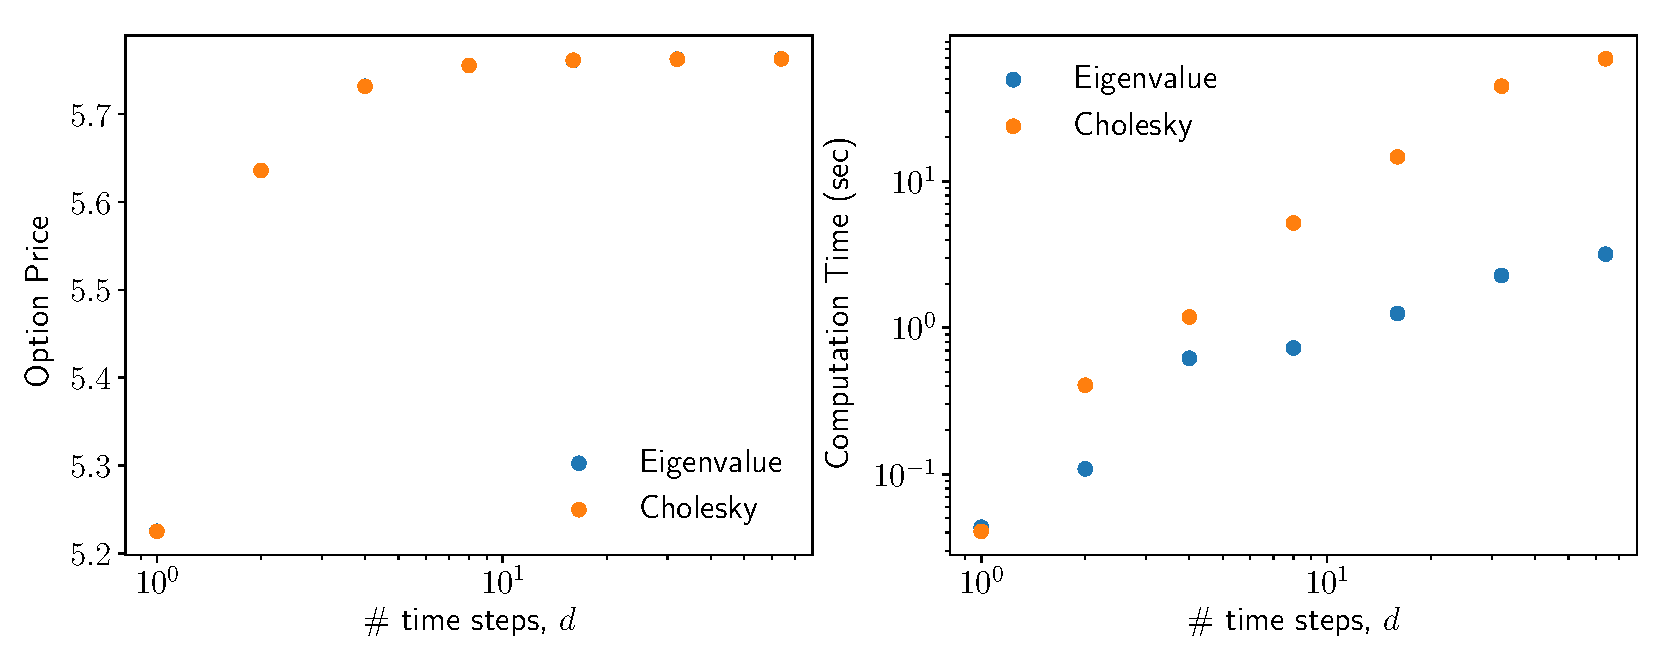
\includegraphics[width=0.8\textwidth]{optionpricing.eps}}

\end{frame}

\begin{frame}{Multilevel methods\footfullcite{Gil14a}}

	\vspace{-5ex}
	Large or infinite $d$ when discretizing a continuous stochastic process.  Write as

	\vspace{-5ex}
	\begin{align*}
		\MoveEqLeft{\lim_{d \to \infty} \int_{[0,1]^d} f_d(\vx_d) \, \dif \vx_d  =
		\overbrace{\int_{[0,1]^{d_1}} f_{d_1}(\vx_{d_1}) \, \dif \vx_{d_1}}^{\text{\alert{low dimensional approximation}}} +
		\overbrace{\int_{[0,1]^{d_2}} [f_{d_2}(\vx_{d_2}) - f_{d_1}(\vx_{d_1}) ]\, \dif \vx_{d_2}}^{\text{\alert{improvement}}} + \cdots }\\
		&
		\quad + \int_{[0,1]^{d_L}} [f_{d_L}(\vx_{d_L}) - f_{d_{L-1}}(\vx_{d_{L-1}}) ]\, \dif \vx_{d_L}
		+ \lim_{d \to \infty} \int_{[0,1]^d} f_d(\vx_d) \, \dif \vx_d -  \int_{[0,1]^{d_L}} f_{d_L}(\vx_{d_L}) \, \dif \vx_{d_L}\\
		& \approx \underbrace{\frac{1}{n_1} \sum_{i=1}^{n_1} f_{d_1}(\vx^{(1)}_{i,d_1})}_{\alert{\text{cheap since } d_1 \text{ small}}}
		+ \frac{1}{n_2} \sum_{i=1}^{n_2} [f_{d_2}(\vx^{(2)}_{i,d_2}) - f_{d_1}(\vx^{(2)}_{i,d_1}) ] + \cdots
		 + \underbrace{\frac{1}{n_L} \sum_{i=1}^{n_L} [f_{d_L}(\vx^{(L)}_{i,d_L}) - f_{d_{L-1}}(\vx^{(L)}_{i,d_{L-1}}) ]}_{\alert{\text{cheap since } n_L \text{ small}}}
	\end{align*}

	\vspace{-3ex}
	where $d_1 < \cdots < d_L$ and $n_1 > \cdots > n_L$.  Evaluation of $f_d(\vx_d)$ is typically $\Order(d)$.


\end{frame}

\section{End}
\againframe<4>{summary}

\begin{frame}[allowframebreaks]{References}
	\printbibliography
\end{frame}

\end{document}

